% generated by scripts/pkl_to_latex.py
% source PKL : thermal_v1_L6_Ne6_U10_t0p1_mode-uniform_tpall_t2all_tperpall_nmin2_solver-gcg_full_restarts2_iter200_kmax4_tol1em09_cut10_adaptive1_step5_clusteravg1_T0to5_N40-205b87919d2f_knone_diag0.pkl
% scan type  : Tscan
% state      : gs
% requires   : \usepackage{pgfplots} \pgfplotsset{compat=1.18}
% colours match the matplotlib PDF (tab10 cycle)
\definecolor{gmeC0}{HTML}{1F77B4}
\definecolor{gmeC1}{HTML}{FF7F0E}
\definecolor{gmeC2}{HTML}{2CA02C}
\definecolor{gmeC3}{HTML}{D62728}
\definecolor{gmeC4}{HTML}{9467BD}
\definecolor{gmeC5}{HTML}{8C564B}
\definecolor{gmeC6}{HTML}{E377C2}
\definecolor{gmeC7}{HTML}{17BECF}

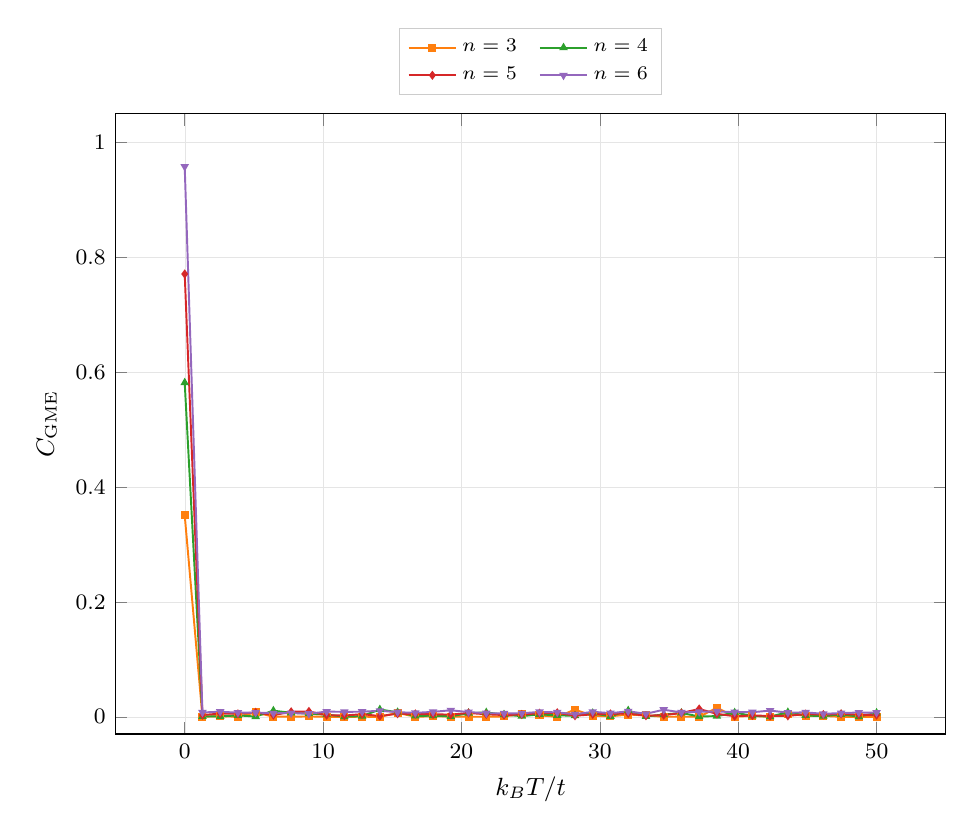
\begin{tikzpicture}
  \begin{axis}[
    width=\columnwidth,
    height=0.78\columnwidth,
    xlabel={$k_B T/t$},
    ylabel={$C_{\mathrm{GME}}$},
    grid=both,
    grid style={line width=.1pt, draw=gray!20},
    tick label style={font=\footnotesize\rmfamily, /pgf/number format/fixed},
    label style={font=\small\rmfamily},
    scaled ticks=false,
    legend style={font=\scriptsize\rmfamily, draw=gray!40, at={(0.5,1.03)}, anchor=south, /tikz/every even column/.append style={column sep=6pt}},
    legend cell align={left},
    legend columns=2,
    ymin=-0.03,
    ymax=1.05,
  ]
    \addplot[color=gmeC1, mark=square*, mark size=1.1pt, line width=0.7pt] coordinates {
        (0,0.351113) (1.282051,0.000007) (2.564103,0.001216) (3.846154,0.000013)
        (5.128205,0.00758) (6.410256,0.000222) (7.692308,0.000187) (8.974359,0.000667)
        (10.25641,0.000002) (11.538462,0.000001) (12.820513,0.00007) (14.102564,0.000003)
        (15.384615,0.006886) (16.666667,0.000072) (17.948718,0.000911) (19.230769,0.000303)
        (20.512821,0.000107) (21.794872,0.000043) (23.076923,0.000632) (24.358974,0.00504)
        (25.641026,0.00254) (26.923077,0.000003) (28.205128,0.012518) (29.487179,0.001674)
        (30.769231,0.000852) (32.051282,0.003976) (33.333333,0.002388) (34.615385,0.000096)
        (35.897436,0.000192) (37.179487,0.000011) (38.461538,0.015834) (39.74359,0.000376)
        (41.025641,0.001438) (42.307692,0.000091) (43.589744,0.005266) (44.871795,0.001707)
        (46.153846,0.001462) (47.435897,0.00002) (48.717949,0.000029) (50,0.000022)
    };
    \addlegendentry{$n=3$}
    \addplot[color=gmeC2, mark=triangle*, mark size=1.1pt, line width=0.7pt] coordinates {
        (0,0.581869) (1.282051,0.00065) (2.564103,0.000654) (3.846154,0.002535)
        (5.128205,0.000417) (6.410256,0.010608) (7.692308,0.00704) (8.974359,0.005482)
        (10.25641,0.003865) (11.538462,0.000279) (12.820513,0.001334) (14.102564,0.012677)
        (15.384615,0.007942) (16.666667,0.001402) (17.948718,0.002009) (19.230769,0.000717)
        (20.512821,0.006472) (21.794872,0.007587) (23.076923,0.003829) (24.358974,0.001068)
        (25.641026,0.004328) (26.923077,0.002391) (28.205128,0.002019) (29.487179,0.006337)
        (30.769231,0.000804) (32.051282,0.010924) (33.333333,0.000656) (34.615385,0.003987)
        (35.897436,0.006678) (37.179487,0.0006) (38.461538,0.001196) (39.74359,0.007268)
        (41.025641,0.001744) (42.307692,0.000353) (43.589744,0.007933) (44.871795,0.002277)
        (46.153846,0.001096) (47.435897,0.004177) (48.717949,0.000474) (50,0.006819)
    };
    \addlegendentry{$n=4$}
    \addplot[color=gmeC3, mark=diamond*, mark size=1.1pt, line width=0.7pt] coordinates {
        (0,0.771122) (1.282051,0.003119) (2.564103,0.005624) (3.846154,0.005172)
        (5.128205,0.007665) (6.410256,0.003024) (7.692308,0.008709) (8.974359,0.009399)
        (10.25641,0.002956) (11.538462,0.002189) (12.820513,0.004591) (14.102564,0.00133)
        (15.384615,0.005383) (16.666667,0.00506) (17.948718,0.00434) (19.230769,0.00388)
        (20.512821,0.00667) (21.794872,0.004415) (23.076923,0.003076) (24.358974,0.004008)
        (25.641026,0.00625) (26.923077,0.006954) (28.205128,0.001885) (29.487179,0.004261)
        (30.769231,0.005075) (32.051282,0.005674) (33.333333,0.001905) (34.615385,0.002886)
        (35.897436,0.006565) (37.179487,0.013661) (38.461538,0.005126) (39.74359,0.001012)
        (41.025641,0.002307) (42.307692,0.001521) (43.589744,0.001594) (44.871795,0.004788)
        (46.153846,0.003845) (47.435897,0.005163) (48.717949,0.003657) (50,0.002928)
    };
    \addlegendentry{$n=5$}
    \addplot[color=gmeC4, mark=triangle*, mark size=1.1pt, mark options={rotate=180}, line width=0.7pt] coordinates {
        (0,0.958179) (1.282051,0.007572) (2.564103,0.00884) (3.846154,0.007184)
        (5.128205,0.007473) (6.410256,0.0062) (7.692308,0.006519) (8.974359,0.005402)
        (10.25641,0.009054) (11.538462,0.008656) (12.820513,0.008858) (14.102564,0.010543)
        (15.384615,0.00805) (16.666667,0.006904) (17.948718,0.008624) (19.230769,0.011365)
        (20.512821,0.008216) (21.794872,0.00631) (23.076923,0.00601) (24.358974,0.006212)
        (25.641026,0.008446) (26.923077,0.007792) (28.205128,0.004415) (29.487179,0.008749)
        (30.769231,0.006363) (32.051282,0.00958) (33.333333,0.005274) (34.615385,0.012313)
        (35.897436,0.007604) (37.179487,0.008704) (38.461538,0.009355) (39.74359,0.008035)
        (41.025641,0.007998) (42.307692,0.010801) (43.589744,0.007288) (44.871795,0.007718)
        (46.153846,0.00521) (47.435897,0.006498) (48.717949,0.007477) (50,0.007292)
    };
    \addlegendentry{$n=6$}
  \end{axis}
\end{tikzpicture}
